\documentclass{article}
\usepackage[utf8]{inputenc}
\usepackage[margin=2cm]{geometry}
\usepackage[style=authoryear]{biblatex}
\usepackage{graphicx}
\addbibresource{bibliography.bib}
\graphicspath{ {img/} }

\title{IMY320 Website Design Proposal: Lona - Realm of Colors}
\date{August 2017}

\begin{document}
\makeatletter
    \begin{titlepage}
        \begin{center}
            
\includegraphics[width=0.7\linewidth]{up.png}\\[4ex]
            {\huge \bfseries \@title }\\[2ex]
            {\LARGE \textbf{Team:} Loners}\\[2ex]
            {\LARGE \@date}\\[2ex]
            {\large  Ritesh Doolabh\\ \texttt{u15075754@tuks.co.za}}\\[2ex] 
            {\large  Jaco du Plooy\\ \texttt{u15226183@tuks.co.za}}\\[2ex]
            {\large  Andreas Nel\\ \texttt{u15066194@tuks.co.za}}\\[2ex] 
            {\large  Brent Walsh\\ \texttt{u15300201@tuks.co.za}}\\[2ex]
        \end{center}
        
    \end{titlepage}
\makeatother
\cleardoublepage
\thispagestyle{empty}
\newpage
\tableofcontents
\newpage
\section{Introduction}
The goal of this document is to propose a design for a website to market and introduce the game, \textit{Lona - Realm of Colors} (\cite{lonaweb}). It is a puzzle game about Lona's journey to explore herself and her past, as seen through the artist's (the player) eyes. The official overview as seen on the game's website is (\cite{lonaweb}):
    \begin{quotation}
    \textit{
    Take the brush as Lona, a young girl on a journey to the deepest depths of herself. Beware though! For in the realm of colors the craving to explore can turn to a yearning to return in a blink of an eye.
    Lona - Realm of Colors is an independent puzzle-adventure dwelling in the highly stylized and abstract past memories of Lona.
    Who is Lona? How did she come to be here? Push fear aside and command the paintings as the original artist, shifting the world to reveal the answers. Discover Lona’s past. Escape the Realm of Colors. Return to reality.}
    \end{quotation}
    
Our choice of design is mainly based on the concept of material design (\cite{materialdesign}). Additionally, the website will be designed in a manner consistent with how the game looks during gameplay, by using some characters, colours and techniques from the game in order to give the user the same look and feel as experienced while playing the game. In the case of elements of the website that are not explained in detail, assume that the standard guidelines as published by Google for Material Design (\cite{materialdesign}) will be followed.

\section{Overview}
The website will consist out of the following pages:
\begin{itemize}
    \item Loading page
    \item Home page
    \item Gallery
    \item Features of the Game
    \item About section
\end{itemize}

Due to the nature of the game and current market trends, we felt that the website would benefit by incorporating the following features into each page, which will be explained further on in the document:
\begin{itemize}
    \item Animation of different elements.
    \item Ability to switch between a light and a dark theme.
    \item A consistent look for each page.
    \item An animation that randomly appears and may possibly interact with the cursor.
\end{itemize}

    \subsection{Layout of Web Pages}
        \begin{flushleft}
        The website will be served in a unique manner whereby the user will have the view of a table (the Frame) and a sheet of art paper (the Page). The user will also have a slightly obstructed view of Lona whose hands will be slightly visible to the user. The sheets of paper symbolize the different web pages that can be viewed. The symbolic nature of the paper indicates that the website is a form of art just as the game is. Each of the different web-pages will be linked with sticky note tabs on the pages. A unique way of scrolling will be implemented whereby the page will only scroll within the paper that is displayed (\cite{youtube_Lona}).
        \bigskip
        \begin{figure}[h]
        \centering
        \caption{Table with paper (inspiration for the framing of each web page) (\cite{youtube_Lona}) }
        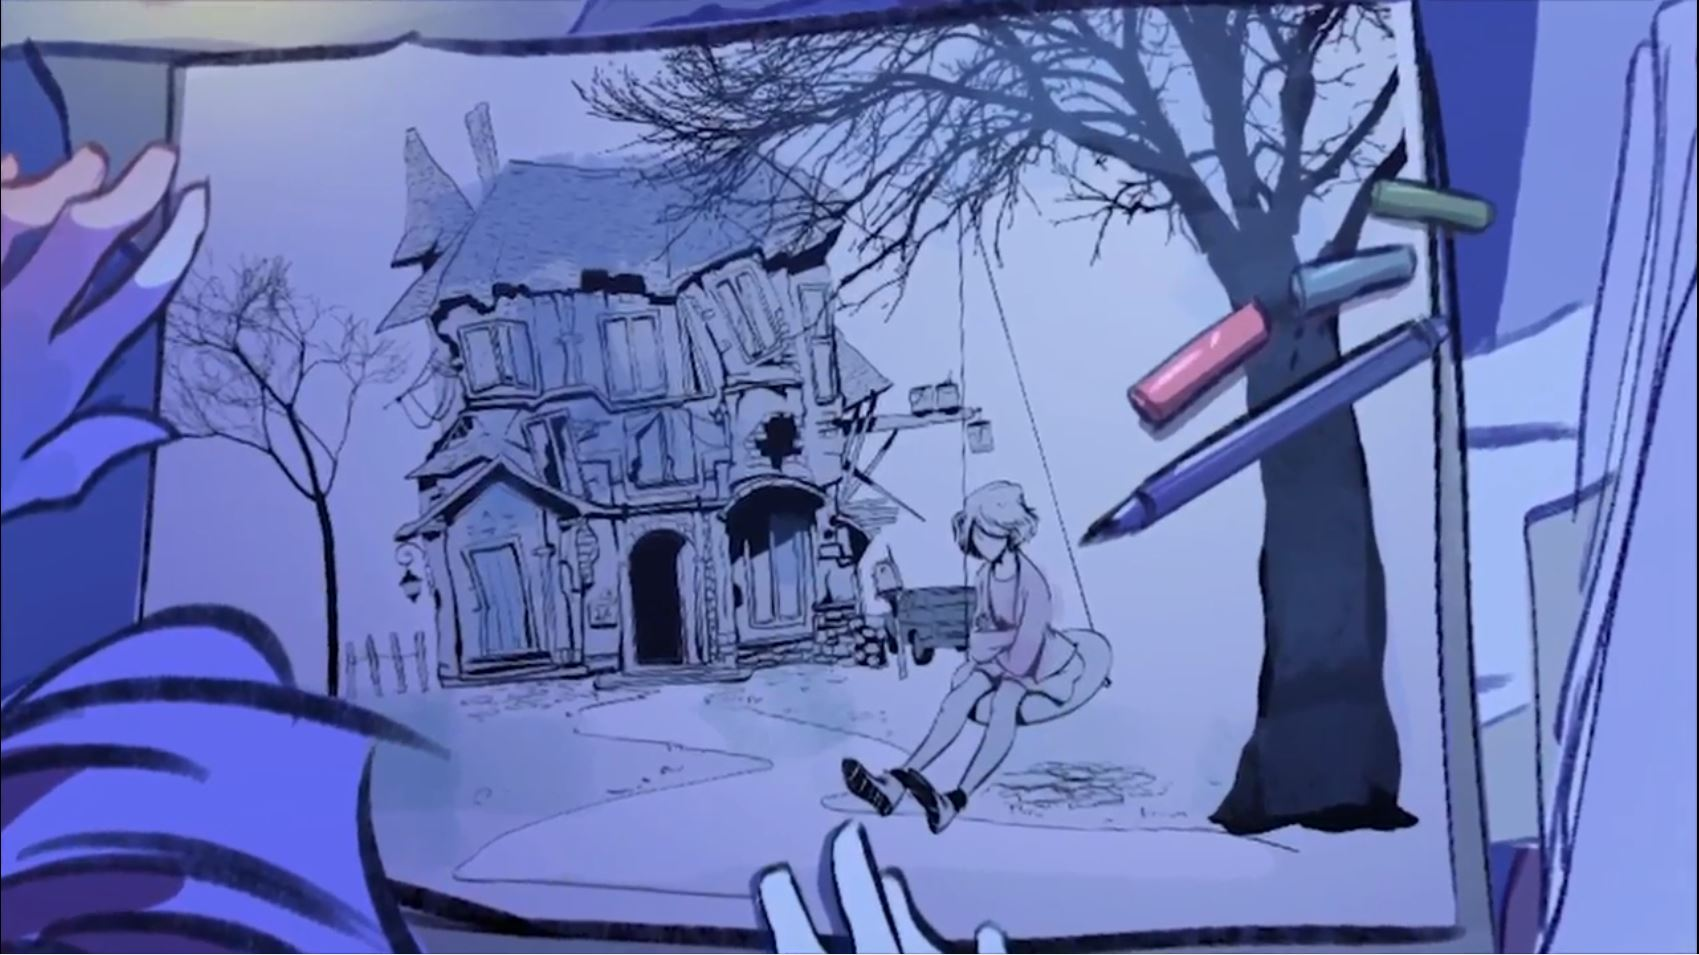
\includegraphics[width=350px]{Table.JPG}
        \end{figure}
        \end{flushleft}
    
    As shown in the concept images in Appendix 1, each page will have a set of colourful buttons that are used to link to each page. The button that represents the page that the user is currently viewing will be wider than the other buttons and will also have extra padding, to create the illusion that each button is a colorful label that is attached to the relevant page. A light will be present in the top-left corner of the Frame, which will then be used to toggle between a light and a dark theme, similar to the actual gameplay of the game (\cite{lonaweb}).
    
    \subsection{Buttons}
    We have decided to make use of raised buttons, a standard type of button in material design that is used to indicate a certain function (\cite{materialize}).
    
    \subsection{Paper}
    The background of the Page will look very similar to the realistic look of paper, as is one of the principles of material design (\cite{principles}). The transition between different pages will happen quickly and seamlessly (if a page struggles to load, the required amount of space required for the Page will still be kept for it so that elements on the screen are not jarred or suddenly moved when the Page finally loads), so that users will not be frustrated with the workflow of the website (\cite{choreography}).
    
    \subsection{Gallery}
    The gallery of the website will be the one page that differs most from the other pages in context of the contents of the Page. The gallery will consist of a bunch of images and videos of concept art and gameplay that is each represented by a card (\cite{cards}) in the left-hand section of the Page. As soon as the user clicks on such a tile, it will expand to the right to give the user a much more detailed and higher quality display of the tile.
    

\section{Animation}
\begin{flushleft}
For our website, we plan to use various subtle, but very effective animations from progress bars to paper stickers. These animations will be present from the first time the website is loaded up all the way through to normal interaction of switching between different web page sections. In addition we will make these animations interactive for the user as they progress to use the website. The animations will be orientated at consuming the user in a world of art and colors (\cite{kickstarter}).
\bigskip

The animations in the website will include all the characters that are present in the game as well as expressing all of their characteristics through this interaction. 
\bigskip

    \subsection{Loading Page}
    First and foremost, the loading page for the website will start showing an animated image of Lona floating up and down with the wind blowing in her hair, as can be seen in the video on the authors' Kickstarter page (\cite{kickstarter}). Around her there will appear colourful swirling teardrops that move up around her body from the bottom indicating zero percent loaded up until the top which indicates the page being fully loaded. In addition to this, the part of Lona's body below the swirling tear-drops will be rendered in color, whereas the part above it will be rendered in grey-scale. This serves to intuitively indicate the loading of the page as well as subtly indicating that the game is centered around art and colours. 
    
    \bigskip
    \begin{figure}[h]
    \centering
    \caption{Lona and the Tear Drops (inspiration for a loading bar) (\cite{youtube_Lona})} 
    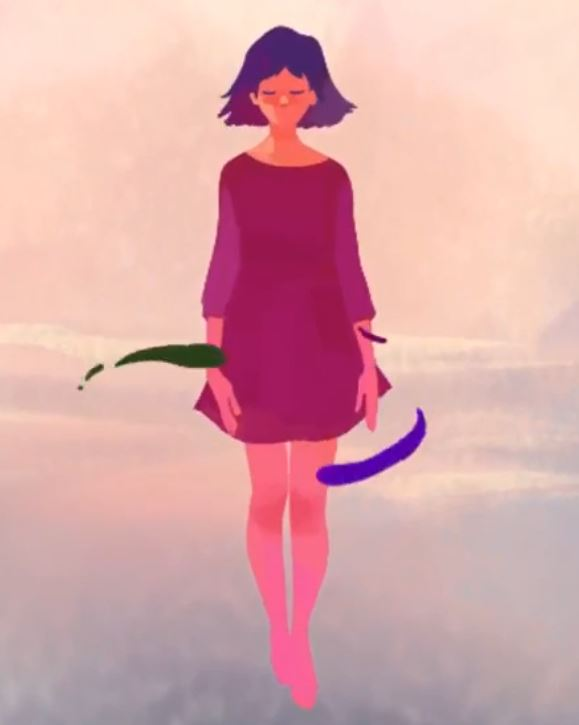
\includegraphics[width=150px]{Lona_loading_bar.JPG}
    \end{figure}
    
    As soon as the loading bar has finished, the figure of Lona will appear to jump backwards, as if she is somersaulting into the page on which she appears. A ripple effect will then introduce the content of the home page and initialize all the figures that appear around the Page, such as the hands, light, buttons, and drawing tools.

    \subsection{General Layout}
    We aim to keep the animation across the whole website consistent, and thus there won't be many unique animations appearing on the different pages, except when specified otherwise. The following animations will however be present at all times:
    \begin{itemize}
        \item The light will always emit a glow that will pulse and change colour, based on the current theme selection.
        \item The hands at the bottom will make slight movements when moused over, to indicate awareness of their surroundings.
        \item When clicking on one of the buttons to move to another page, Lona's hands will quickly move to the general button area and swipe the page away, as if discarding it, in order to reveal the new web page underneath it.
        \item There will at random times appear an animation of a white cat (or a black crow in the case of a dark theme) that will walk/fly around the Page and appear to take notice of the cursor when the user moves it closer to the character. The character will then appear to be frightened if clicked on and run away, out of the Page to the side. This is purely for aesthetic purposes, but does however introduce the characters of \textit{Mrs Schmidt} (the cat) and \textit{Mr Ruppel} (the crow) (\cite{kickstarter}).
    \end{itemize} 
\end{flushleft}

\section{Colours}
    \begin{flushleft}
    The colour scheme of the website will be taken from the colour palette of the game itself. This encompasses bright and vivid colours for the light theme, and somber and monotone for the dark theme (\cite{kickstarter}). This is inspired by the game's usage of both a light and a dark side for each level that is used to introduce different aspects to the gameplay. The warm and bright colour scheme will be opposed with the dark monotone of the dark side when chosen. For this we will make use of different shades of dark and cold colours to show the dark side.
    \end{flushleft}

    \subsection{Light and Dark}
    \begin{flushleft}
    A two layer theme will be used in conjunction with the website where there will be a dark and light theme available for the user to pick from. This is taken directly from the game where the light side represents the joyfulness and chaos of Lona's art and the dark side represents the somberness and darkness of that same art. The website's colours will be changed accordingly to the option that the user picks. The light and dark themes symbolize Lonas conflicting two emotions and that painting them is her release from being absorbed by them (\cite{lonaweb}).
    \bigskip
    
    \begin{figure}[h]
    \centering
    \caption{Difference in themes in the Game (\cite{lonatwitter})}
    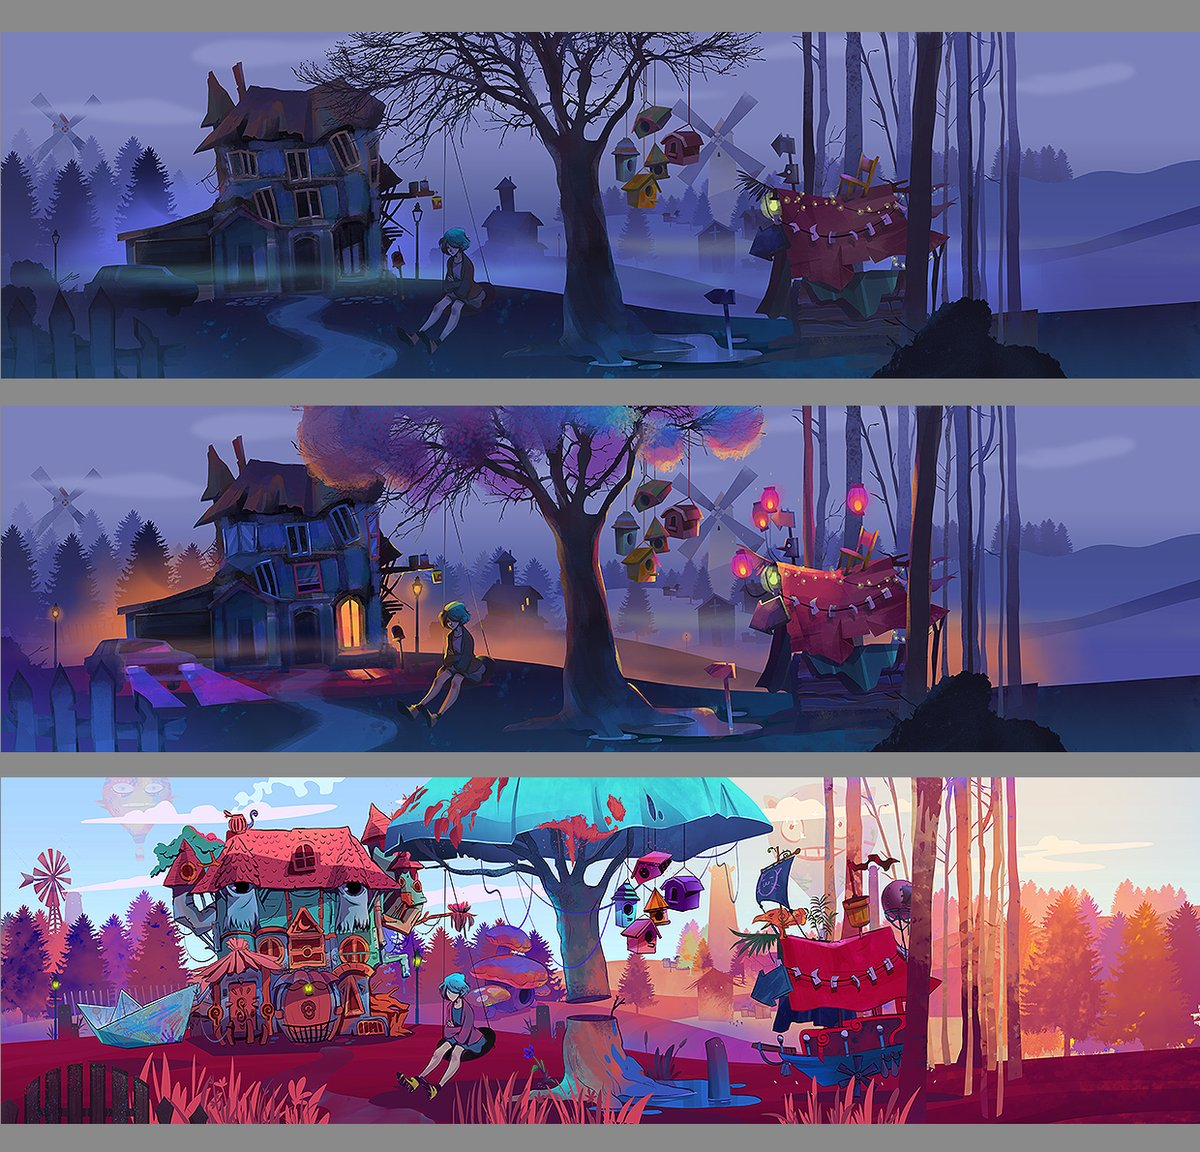
\includegraphics[width=350px]{Theme_Contrast.jpg}
    \end{figure}
    \end{flushleft}

    \subsection{Characters}
    \begin{flushleft}
    The website will incorporate all the different characters that are in the game as well as their respective traits. The characters will appear on different pages and animated in such a way that they portray their roles in the game in a visual manner. This will be done by using the form of colours that each character represents. For example the crow which is part of the dark side (\cite{kickstarter}) will only appear when that theme is selected and the cat which is part of the chaotic side (\cite{kickstarter}) will appear when the light theme is shown. These characters will also be animated such that they exhibit their characteristics, whereby the cat will cause chaos on the canvas, in this case the website. 
    Lona who is the main character will also be shown in a world on her own, and her demeanour transforms from a state of depression into a state of inner peace as more colour is added. 
    \end{flushleft}
    
\newpage
\section{Appendices}
\subsection{Appendix 1: Concept Images}
% concept image of loading bar
    \begin{figure}[h]
    \centering
    \caption{Concept for loading page}
    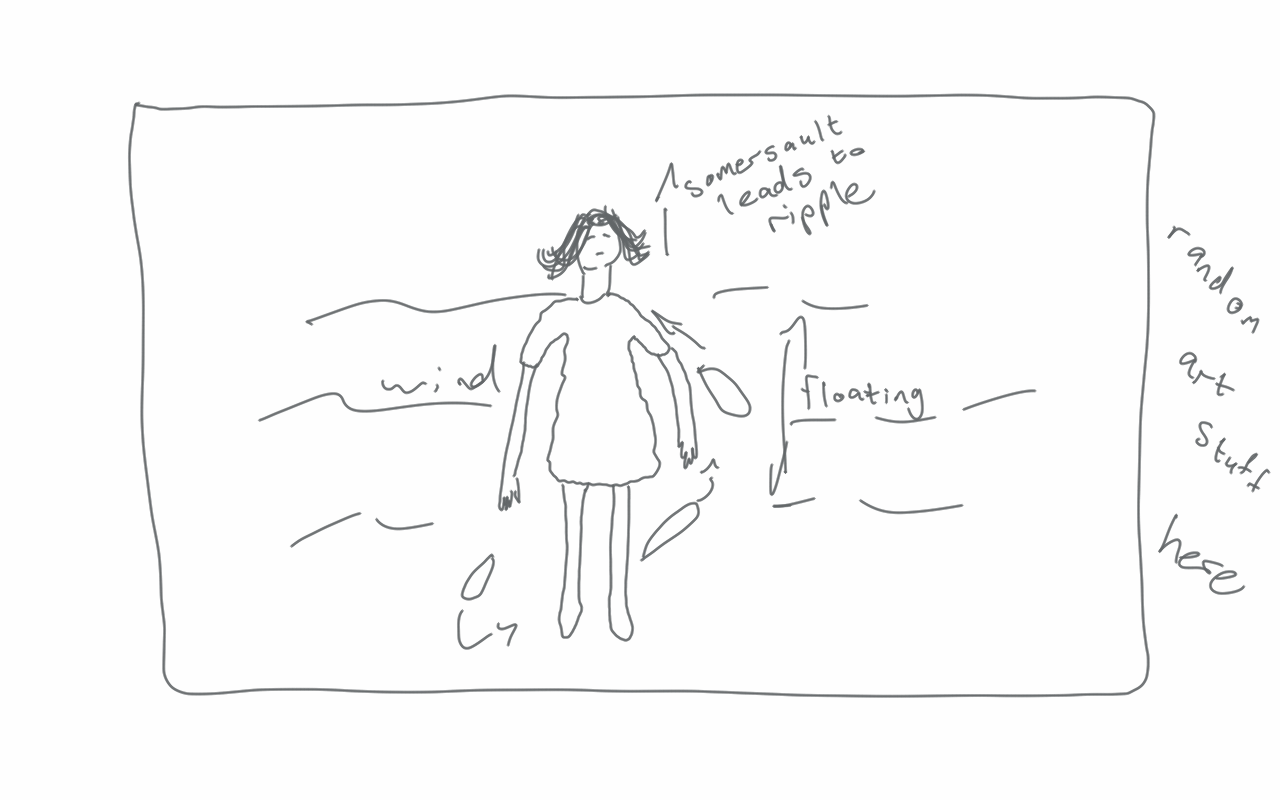
\includegraphics[width=350px]{Concept_Loading.png}
    \end{figure}
% concept image of the frame
    \begin{figure}[h]
    \centering
    \caption{Concept image for general layout of Page}
    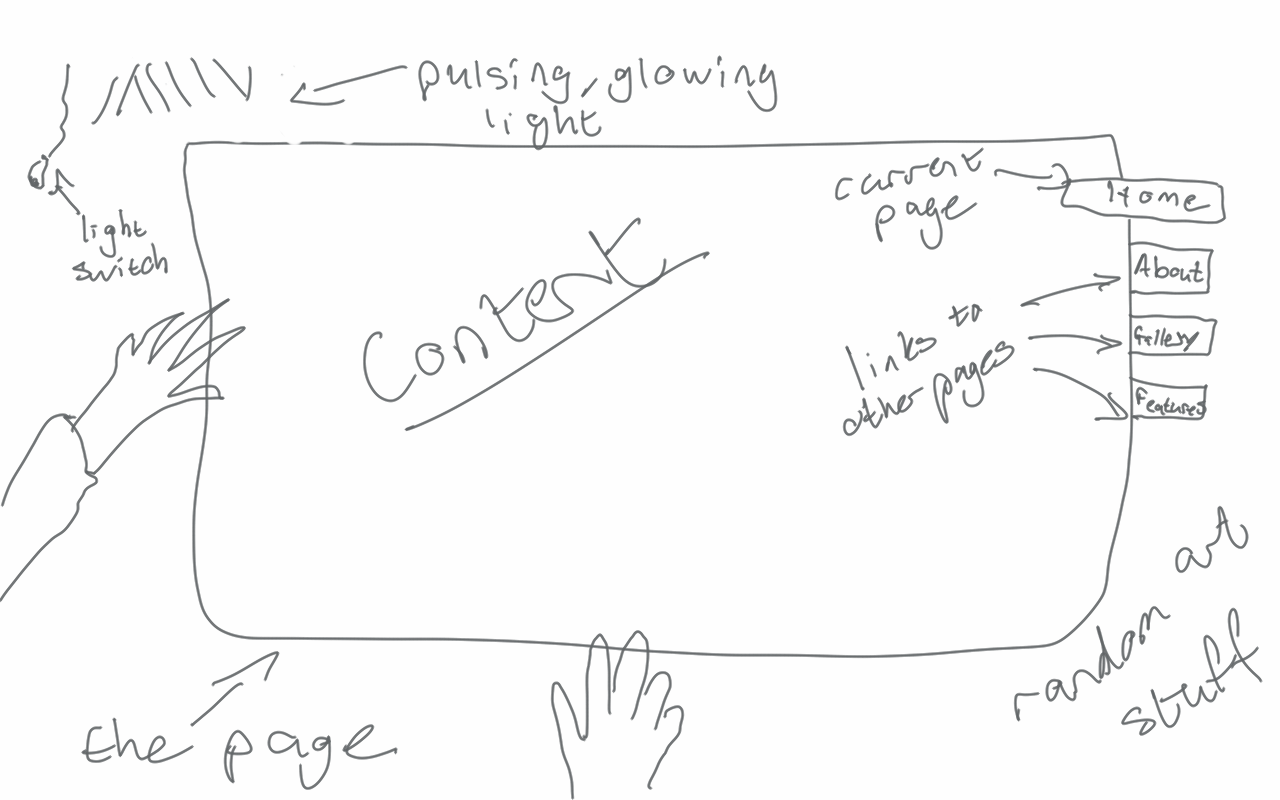
\includegraphics[width=350px]{Concept_Frame.png}
    \end{figure}
% concept image of the gallery
    \begin{figure}[h]
    \centering
    \caption{Concept image for Gallery page}
    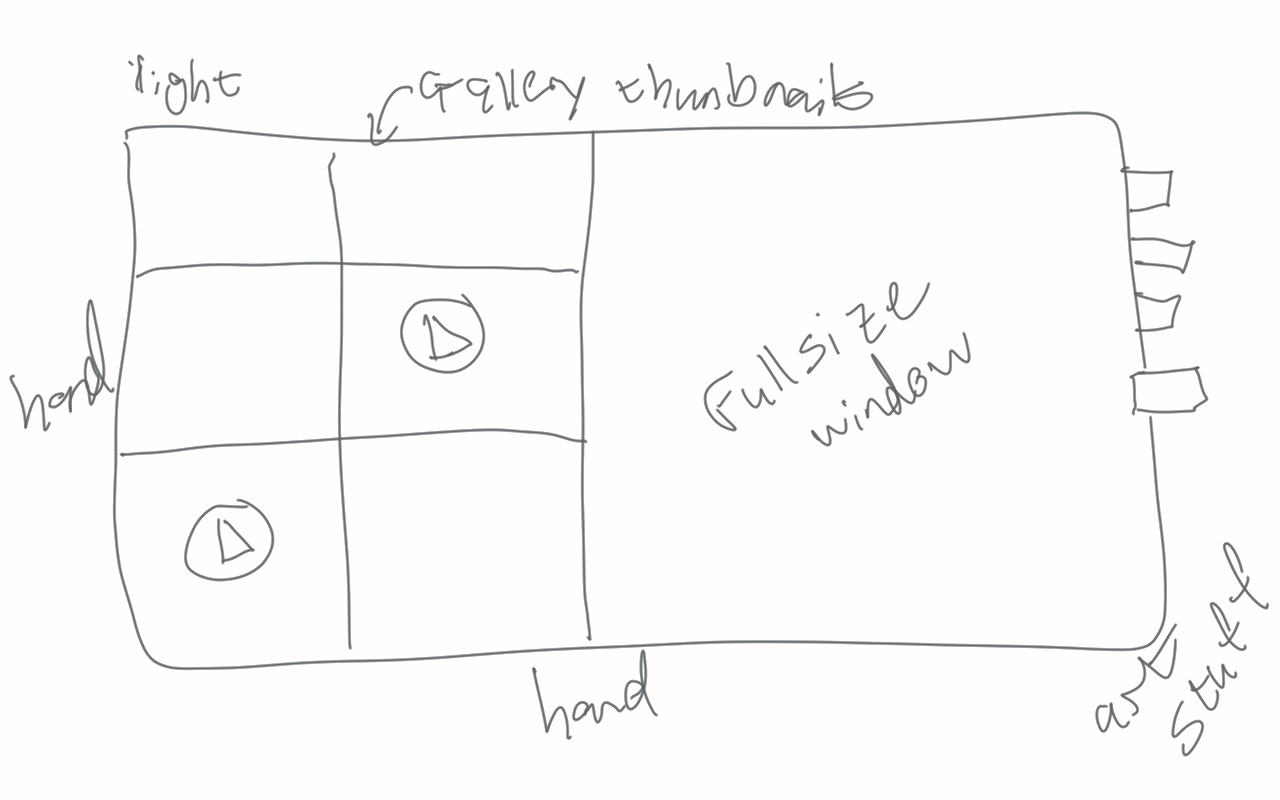
\includegraphics[width=350px]{Concept_Gallery.png}
    \end{figure}
\newpage
\subsection{Appendinx 2: Exhibits}
    \bigskip
    \begin{figure}[h]
    \centering
    \caption{Exhibit of both the bright and the pastel colours that will be used (\cite{youtube_Lona}) }
    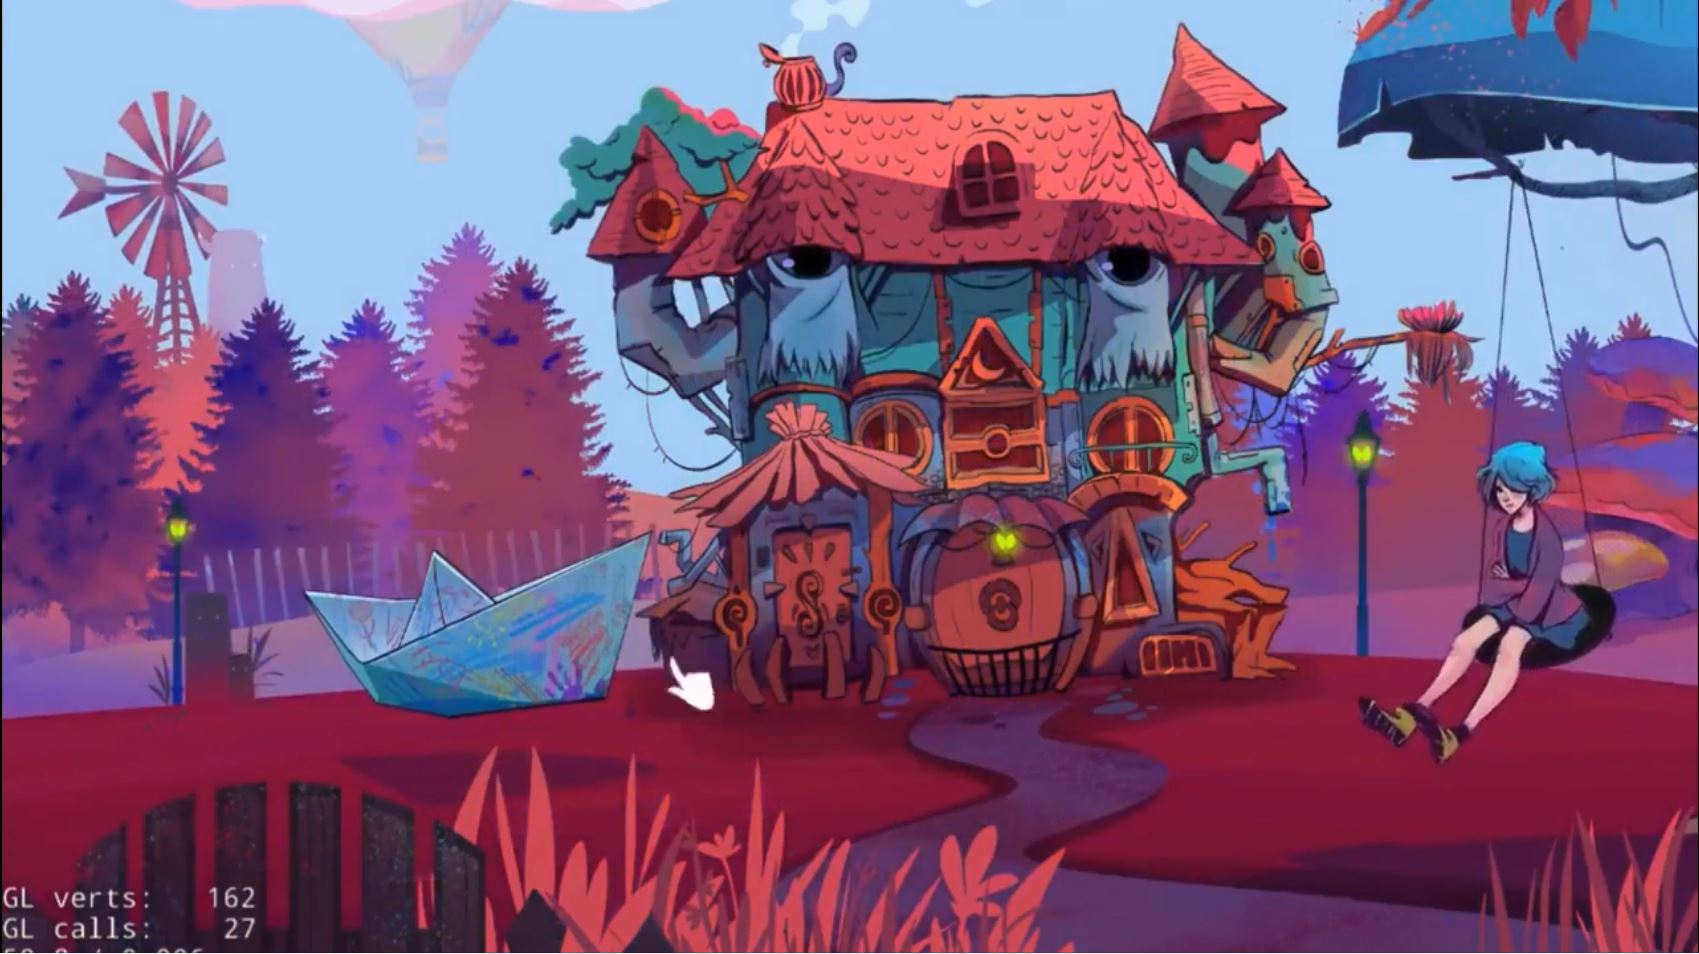
\includegraphics[width=350px]{Colours.JPG}
    \end{figure}
    
    \bigskip
    \begin{figure}[h]
    \centering
    \caption{Exhibit of the dark colours that will be used (\cite{youtube_Lona})}
    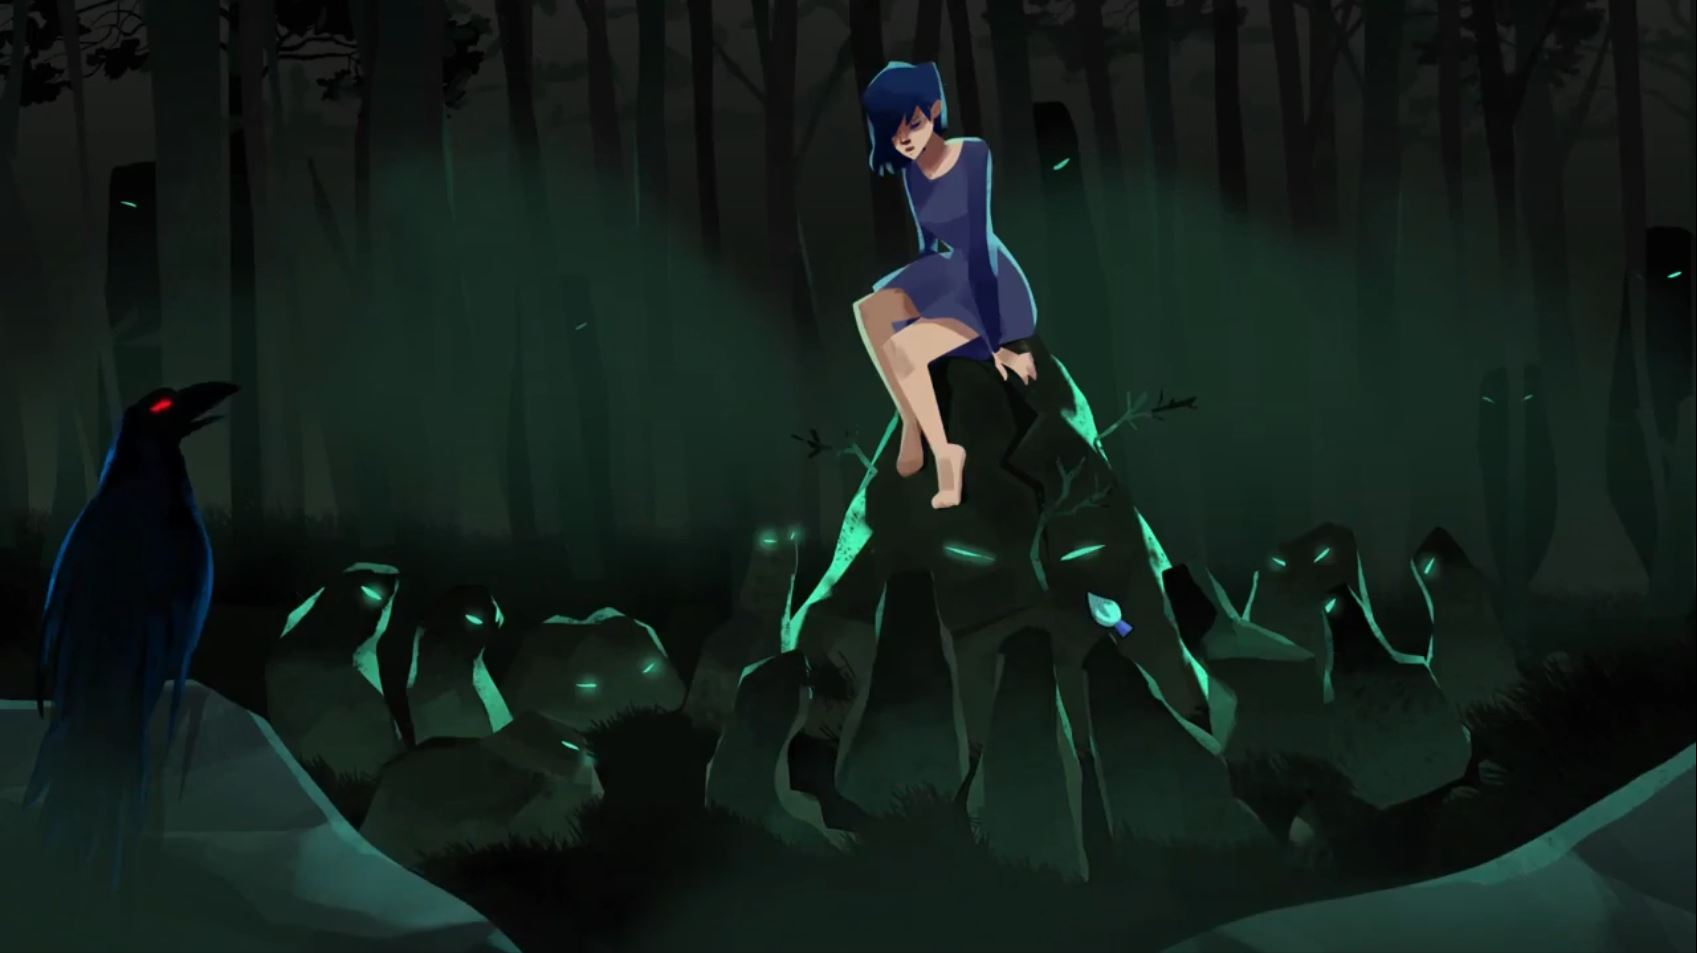
\includegraphics[width=350px]{Dark_Colours.JPG}
    \end{figure}
\newpage
\addcontentsline{toc}{section}{References}
\printbibliography
\end{document}